\documentclass[11pt, letterpaper]{article}
\input{/home/hyperion/.config/LatexHub/preambles/base.tex}
\input{/home/hyperion/.config/LatexHub/preambles/diagrams.tex}
\input{/home/hyperion/.config/LatexHub/preambles/tikz.tex}
\input{/home/hyperion/.config/LatexHub/preambles/macros-cat-theory.tex}
\input{/home/hyperion/.config/LatexHub/preambles/macros-algebra.tex}
\input{/home/hyperion/.config/LatexHub/preambles/basic-theorems-section.tex}
\input{/home/hyperion/.config/LatexHub/preambles/refs-basic.tex}
\theoremstyle{plain}
\newtheorem{problem}{Problem}[section]


\usepackage{titlesec}
\titleformat{\section}{\normalfont\Large\bfseries}{}{0em}{}
\usepackage{titlepageBU}
\usepackage{pgfplots}
\pgfplotsset{compat=1.18}
\title{Homework 3}
\begin{document}
\makeproblem
\section{Problem 4.5}

\begin{problem}
	Show that the quotient $\pi : \mathbb{C} ^{n+1} \setminus \left\{ 0 \right\}  \to \mathbb{C} \mathbb{P} ^n$ is a surjective smooth submersion. Then show $\mathbb{C}\mathbb{P} ^1$ is diffeomorphic to $S^2$.
\end{problem}
\begin{proof}
	We showed previously that $\pi $ was smooth. It's also manifestly surjective, since given any $[x]\in\mathbb{C} \mathbb{P} ^n$, there is at least one representative $x\in\mathbb{C} ^{n+1} \setminus \left\{ 0 \right\} $, and by definition $\pi (x)=[x]$.

	To show $\pi $ is a submersion, we appeal to the local section theorem (Lee 4.26). Let $[x]\in\mathbb{C} \mathbb{P} ^n$ and let $U\subseteq \mathbb{C} \mathbb{P} ^n$ an open neighborhood of $[x]$. Suppose we can define some smooth $\sigma : U \to \mathbb{C} ^{n+1} $ such that for any $[y]\in U$, we map $\sigma [y]=y$ for some representative $y\in[y]$. Then $\sigma $ will be a local section of $\pi $, since $(\pi \circ \sigma )[y]=\pi (y)=[y]$. It suffices to show such a $\sigma $ can be constructed in a smooth manner.

	We specialize to the case where $U=U_i$ is the chart
	\[
		U_i=\pi (\widetilde{U}_i),\qquad \widetilde{U} _i=\left\{ x\in\mathbb{C} ^{n+1} \mid x^i\neq 0 \right\} 
	.\]
	This is sufficient since the charts cover $\mathbb{C} \mathbb{P} ^n$. In homework 1, I showed that the map
	\[
		[x]\mapsto \left( \frac{x^1}{x^i} ,\ldots ,\frac{x^{i-1} }{x^i} ,\frac{x^{i+1} }{x^i} ,\ldots ,\frac{x^n}{x^i}  \right)
	\]
	was smooth $\mathbb{C} \mathbb{P} ^n\to \mathbb{C} ^n$. Since the constant map is smooth, we see that there is a smooth map $\mathbb{C} \mathbb{P} ^n\to \mathbb{C} ^{n+1} $ given by
	\[
		[x]\mapsto \left( \frac{x^1}{x^i} ,\ldots ,\frac{x^{i-1} }{x^i} ,1,\frac{x^{i+1} }{x^i} ,\ldots ,\frac{x^n}{x^i}  \right)
	.\]
	Define $\sigma : \mathbb{C} \mathbb{P} ^n \to \mathbb{C} ^{n+1} $ as this map. In my first homework, I also showed that $\sigma [x]$ was a representative of $[x]$. We repeat the argument here: $\sigma [x]$ is colinear with $x^i\sigma [x]$ since $x^i\neq 0$ by assumption, so
	\[
		x^i\sigma [x]=x^i\left( \frac{x^1}{x^i} ,\ldots ,\frac{x^{i-1} }{x^i} ,1,\frac{x^{i+1} }{x^i} ,\ldots ,\frac{x^n}{x^i}  \right)=\left( x^1, \ldots ,x^n \right) =x
	.\]
	By assumption, $x\in[x]$, so we have that $\sigma [x]$ is a representative of $[x]$, and since $\sigma $ is smooth, the statement follows.

	To show the diffeomorphism, define $F : \mathbb{C} \mathbb{P} ^1 \to \mathbb{C} \cup \left\{ \infty  \right\}$ as the map
	\[
		F[x^1,x^2]=
		\begin{cases}
			x^2/x^1,&x^1\neq 0\\
			\infty ,&x^1=0
		\end{cases}
	.\]
	Of course $\mathbb{C} \cup \left\{ \infty  \right\} $ (with antipodal points identified at $\infty $), when given the usual topology, has homeomorphisms $\mathbb{C} \cup \left\{ \infty  \right\} \cong \mathbb{R} ^2 \cup \left\{ \infty  \right\} \cong S^2$; the first isomorphism is given by the usual identification $\mathbb{C} \cong \mathbb{R} $, and the second is given by stereographic projection, where we identify $\infty $ with the north pole and project the south pole to $0$. I'm out of time to submit the homework, but the proof should proceed as follows:
	\begin{enumerate}
		\item First, promote $\mathbb{C} \cup \left\{ \infty  \right\} $ to a smooth manifold in such a way that is compatible with the smooth structure on $\mathbb{C} $. We then induce an analogous smooth structure on $\mathbb{R}^2 \cup \left\{ \infty  \right\} $:q

		\item We will then show this smooth structure is compatible with the stereographic projection, which is already known to be smooth onto $S^2$ with a pole removed. We will then show that inserting $\infty $ as the removed pole is smooth, and thus there is a diffeomorphism $\mathbb{C} \cup \left\{ \infty  \right\} \cong S^2$.
		\item We will finally show $F$ is a diffeomorphism.
	\end{enumerate}
\end{proof}


\section{Problem 4.8}
\begin{problem}
	Let $\pi : \mathbb{R} ^2 \to \mathbb{R} $ be the map $\pi (x,y)=xy$. Show that $\pi $ is surjective and smooth, and for each smooth manifold $P$, a map $F : \mathbb{R}  \to P$ is smooth if and only if $F\circ \pi $ is smooth. Then show $\pi $ is not a submersion.
\end{problem}
\begin{proof}
	Becauase charts on $\mathbb{R} ^n$ are simply the identity map, $\pi $ is smooth if it is smooth in the calc 3 sense. This follows immediately:
	\[
		\frac{\partial \pi }{\partial x} =y,\qquad \frac{\partial ^2\pi }{\partial x^2} =0,\qquad \frac{\partial \pi }{\partial y} =x,\qquad \frac{\partial^2 \pi }{\partial y^2} =0,\qquad \frac{\partial ^2\pi }{\partial x \partial y} =1
	.\]
	To show surjectivity, let $x\in\mathbb{R} $, and note that $\pi (x,1)=x$. Thus, $\pi (\mathbb{R} \times \left\{ 1 \right\} )=\mathbb{R} $, and the map is surjective.


	To show the second part, note that if $F$ is smooth, then $F\circ \pi $ is smooth because it is a composite of smooth functions. For the converse, let $F\circ \pi $ be smooth. Define $i : \mathbb{R}  \to  \mathbb{R} \times \mathbb{R} $ by $x\mapsto (1,x)$. This is smooth since it is smooth componentwise. We claim that restricting $F\circ \pi $ along $i$ recovers $F$:
	\[\begin{tikzcd}[row sep = 2.5em, column sep = 2.5em]
	\mathbb{R} \ar[" i "', r] \ar[" F ", bend left, rrr] & \mathbb{R} \times \mathbb{R} \ar[" \pi  "', r]  & \mathbb{R} \ar[" F "', r]  & \mathbb{R} .
	\end{tikzcd}\]
	Indeed, let $x\in\mathbb{R} $. Following $x$ along this composite yields
	\[\begin{tikzcd}[row sep = 2.5em, column sep = 2.5em]
	x \ar[" i ", mapsto, r]  & (1,x)\ar[" \pi  ", mapsto, r]  & x\ar[" F ", mapsto, r]  & F(x).
	\end{tikzcd}\]
	Therefore, $F=F\circ \pi \circ i$. Since $F\circ \pi $ and $i$ are smooth, we have that $F$ is a composite of smooth maps, and thus smooth.

	Since $\pi $ is surjective, if it has constant rank then it will be a submersion by Lee Thm. 4.14. Thus, $\pi $ must not have constant rank. Since $\pi (-,0)=\pi (0,-)=0$, and $\pi (1,-)=\pi (-,1)=\mathrm{id} $, we might assume that $\pi $ will have different rank at a point containing a 0 versus a point containing a 1 (and no zeroes).

	Since the charts on $\mathbb{R} ^n$ are the identity, the tangent space $T_p\mathbb{R} ^n$ is spanned by the usual derivatives evaluated at $p\in\mathbb{R} ^n$. Consider $p=(1,1)$ and $q=(0,0)$. We consider the action of $\mathrm{d}_{p,q} \pi $ on the basis elements $\partial _x,\partial _y$ of $T_{p,q} \mathbb{R} ^2$. Let $f : \mathbb{R} \to \mathbb{R} $. From our knowledge of calculus, we have
	\[
		\mathrm{d}_p\pi (\partial_x|_p)(f)=\left.\frac{\partial f\circ \pi }{\partial x} \right|_p=\left. \frac{\partial f\circ \pi }{\partial \pi } \frac{\partial \pi }{\partial x} \right|_p=\left.\frac{\partial f}{\partial x} \right|_{\pi (p)} \left.\frac{\partial \pi }{\partial x} \right|_p
	.\]
	Since $\partial_x\pi =y$ and $p=(1,1)$, we have that $\partial_x\pi |_p=1$. Therefore, this evaluates to
	\[
		\left.\frac{\partial f}{\partial x} \right|_{1} 
	.\]
	This is nonzero in general. For example, $f=x^2+x$ has a nonzero derivative at $1$. Therefore, $\mathrm{d} _p\pi $ has nonzero rank.

	For the other point, we also see that
	\[
		\mathrm{d}_q\pi (\partial _x|_q)(f)=\left. \frac{\partial f}{\partial x} \right|_{\pi (q)} \left.\frac{\partial \pi }{\partial x} \right|_q
	.\]
	However, $q=(0,0)$, so $\partial_x\pi =y$ evaluated at $0$ is $0$. Therefore,
	\[
		\mathrm{d}_q\pi (\partial _x|_q)=0
	.\]
	Since $\partial _y\pi =x$, we see that $\mathrm{d}_q\pi (\partial _y|_q)$ is also zero. Therefore, the rank of $\mathrm{d}_q\pi $ is zero, and $\pi $ does not have constant rank.
\end{proof}

\section{Problem 4.10}
\begin{problem}\label{3}
	Show that the map $q : S^n \to \mathbb{R} \mathbb{P} ^n$ given by the composite
	\[\begin{tikzcd}[row sep = 2.5em, column sep = 2.5em]
		q: S^n\ar[" \iota  ", hook, r]  & \mathbb{R} ^{n+1} \ar[" \pi  ", r]  & \mathbb{R} \mathbb{P} ^n
	\end{tikzcd}\]
	is a smooth covering map.
\end{problem}
\begin{proof}
	Since we have already shown $\pi $ is smooth and since the inclusion is very clearly smooth, we have that $q$ is smooth. Recall that a subset $U \subseteq \mathbb{R} \mathbb{P} ^n$ is open if and only if $\pi ^{-1} (U)$ is open in $\mathbb{R} ^{n+1} \setminus \left\{ 0 \right\} $ by definition of the quotient topology. The preimage $(\pi \circ \iota )^{-1} (U)$ is simply the restriction of $\pi^{-1} (U)$ along $S^n$, meaning
	\[
		(\pi \circ \iota )^{-1} (U)=\pi ^{-1} (U)\cap S^n
	.\]
	Let $[x]\in \mathbb{R} \mathbb{P}^n$, and choose a representative $x\in\mathbb{R} ^{n+1} $ of $[x]$. For simplicity, choose $x$ such that $\left| x \right| =1$. For simplicity once again, take $0<r<1$, and consider the set $U\coloneqq q(B_r(x)\cap S^n)\subseteq \mathbb{R} \mathbb{P} ^n$. We claim that $q^{-1} (U)$ has two components:
	\[
		q^{-1} (U)=(B_r(x) \cap S^n) \cup (B_r(-x) \cap S^n)
	.\]

	First, we prove that $U$ is an open neighborhood of $[x]$. The fact that $[x]\in U$ is simple, since $x$ has norm 1, meaning $x\in S^n$, and thus $x\in S^n \cap B_r(x)$. We thus have $q(x)=[x]\in U$. To show $U$ is open, we must show the preimage $\pi ^{-1}(U)$ is open. The proof is an annoying yet routine verification, so we simply note that the preimage is a double cone that does not contain its boundary, so given a point we can always choose a distance such that the ball about that point falls within the double cone.

	Now we prove the claimed equality. Let $p\in B_r(x) \cap S^n$. Then $q(p)=[p]\in U$, and $q^{-1} [p]=[p]\cap S^n=\left\{ p,-p \right\} $, where we have noted that since the span of $p$ is a one-dimensional space, it has preciely two unit vectors, $p$ and $-p$. Since $p\in q^{-1} [p]\subseteq q^{-1} (U)$ and $-p\in q^{-1} [p]\subseteq q^{-1} (U)$, we have $B_r(x) \cap S^n \subseteq q^{-1} (U)$ and $B_r(-x) \cap S^n \subseteq q^{-1} (U)$. For the converse, let $p\in q^{-1} (U)$. Then $p\in S^n$ by hypothesis. Additionally, $[p]\in U$ implies that there is some $q\in [p]$ with $q\in B_r(x) \cap S^n$. However,since the span of $p$ is a one-dimensional space, there are precisely two unit vectors, $p$ and $-p$. We thus have $p=q\in B_r(x)$ (without loss of generality), and thus $-p\in B_r(-x)$. Therefore,
	\[
		q^{-1} (U)=(B_r(x) \cap S^n) \cup (B_r(-x)\cap S^n)
	.\]
	Note that the distance $d(x,-x)=\left| x+x \right| =2\left| x \right| =2$. Since $r<1$, we thus have that $B_r(x),B_r(-x)$ are disjoint, since any $p\in B_r(x)$ has $d(p,x)<1$ and thus $d(p,-x)>1$. Therefore, the sets are disjoint. It should be clear that they are connected since they are simply arcs of circles.

	We claim that restricting $q$ along $B_r(x)$, and equivalently restricting $\pi $ along $B_r(x)\cap S^n$, is a diffeomorphism $B_r(x) \cap S^n \cong U$. Indeed, recall that given $[p]\in\mathbb{R} \mathbb{P} ^n$, there are \emph{precisely two} representatives $p^+,p^-$ in $S^n$; we define $p^+$  to be the representative in $B_r(x)$ and $p^-$ the one in $B_r(-x)$. The inverse to the restriction $q|B_r(x) \cap S^n$ is then given by $[p]\mapsto p^+$, and similarly for $B_r(-x) \cap S^n$, the inverse is $[p]\mapsto p^-$. These maps are inverses by the uniqueness of the representative of $[p]$ in $B_r(x) \cap S^n$. Write $\psi $ for the inverse of $q$ on $B_r(x) \cap S^n$. We of course have that $q$ is smooth on $B_r(x) \cap S^n$ since it is smooth globally, so it suffices to show $[p]\mapsto p^+$ is smooth. The logic for the $[p]\mapsto p^-$ case is equivalent.

	Since $x\in S^n$, it has at least one nonzero component. Take $x^i$ to be this component. It follows that there is some nonzero $d$ defined as the smallest distance to a point on $S^n$ with $x^i=0$:
	\[
		d\coloneqq \min \left\{ d(x,y)\mid y^i=0 \right\} >0
	.\]
	Earlier we chose $0<r<1$. We now modify our choice of $r$ such that $0<r<d$ and $0<r<1$. Of course taking $r$ this small does not change any of the above logic, since it only relied on the fact that $0<r<1$ which is still true. By definition  of $d$, we have that each $y\in B_r(x)$ has $y^i \neq 0$, and thus $B_r(x)\subseteq \widetilde{U}_i$, where we recall
	\[
		\widetilde{U}_i \coloneqq \left\{ y\in\mathbb{R} ^{n+1} \setminus \left\{ 0 \right\} \mid y^i \neq 0 \right\} 
	.\]
	Recall also that the chart $U_i$ on $\mathbb{R} \mathbb{P} ^n$ is defined as $\pi (\widetilde{U}_i)$, and thus we have $U=q(B_r(x) \cap S^n)$ is a subset of the chart $U_i$. The chart $\mathbb{R} ^{n}  \to U_i$ is defined by the map $\varphi ^{-1} :\mathbb{R} ^n\to U_i$ given by
	\[
		x\mapsto [y^1, \ldots ,y^{i-1} ,1,y^{i} ,\ldots ,y^n].
	\]
	Take $y^i>0$ without loss of generality (since if $y^i<0$, we pass to the $B_r(-x)$ case which follows by the same logic). Then all $y\in B_r(x) \cap S^n$ has $y^i>0$ by the intermediate value theorem, and thus $B_r(x) \cap S^n$ is a subset of $U^+_i$, which we recall is given by
	\[
		U_i^+ \coloneqq \left\{ y\in S^{n} \mid y^i>0 \right\} 
	.\]
	The chart $\varphi^+_i : U_i \to \mathbb{R} ^{n} $ is given by
	\[
		y\mapsto (y^1, \ldots ,y^{i-1} ,y^{i+1} ,\ldots ,y^n)
	.\]
	We now want to show the map $\varphi ^+_i \circ \psi \circ \varphi_i^{-1} $ is smooth. First, note that
	\[
		\varphi _i ^{-1} :y\mapsto [y^1, \ldots ,y^{i-1} ,1,y^{i} ,\ldots ,y^n].
	\]
	We want to normalize the given representative to find the element of $B_r(x) \cap S^n$ (we have implicitly taken $y$ such that its image is inside $U$). We thus have
	\[
		[y^1, \ldots ,y^{i-1} ,1,y^{i} ,\ldots ,y^n]=\frac{1}{\sqrt{(y^1)^2+\cdots (y^n)^2+1} } \varphi _i^{-1} (y)=\frac{\varphi _i^{-1} (y)}{\sqrt{1+\left| y \right| } } 
	.\]
	The given representative is now of unit norm, and since we have without loss of generality taken $y^i>0$, we have
	\[
		\psi : \frac{\varphi_i ^{-1} (y)}{\sqrt{1+\left| y \right| } } \mapsto \frac{(y^1, \ldots ,y^{i-1} ,1,y^{i} ,\ldots ,y^n)}{\sqrt{1+\left| y \right| } } 
	.\]
	Mapping along $\varphi_i^{+} $ gives
	\[
		\frac{1}{\sqrt{1+\left| y \right| } } y
	.\]
	Thus, the composite $\varphi _i^+\circ \psi \circ \varphi_i^{-1} $ is simply multiplication by $\left( 1+\left| y \right|  \right)^{-1/2}  $. Since this is a composite of smooth functions, it is indeed smooth, and thus $q$ has a smooth inverse along the component.
\end{proof}

\section{Problem 4.13}

\begin{problem}
	Let $F : S^2 \to \mathbb{R} ^4$ be the map $F(x,y,z)=(x^2-y^2,xy,xz,yz)$. Using the covering in \cref{3}, show that $F$ descends to a smooth embedding $\mathbb{R} \mathbb{P} ^2\hookrightarrow \mathbb{R} ^4$.
\end{problem}
\begin{proof}
	By Lee 4.33, $q : S^2 \to \mathbb{R} \mathbb{P} ^2$ is a quotient, and thus by universality of quotient (Lee 4.30), if $F$ is constant on fibers of $q$, then it descends along $q$ to a well-defined map $\mathbb{R} \mathbb{P} ^2\to \mathbb{R} ^4$. We must show that it indeed descends, and then we must show that the induced map is a smooth embedding.

	First, recall from \cref{3} that each $[x,y,z]\in\mathbb{R} \mathbb{P} ^2$ has precisely two preimages in $S^2$ under $q$, which we denoted $(x,y,z)^+$ and $(x,y,z)^-$. Of course we just chose these labels based on some choice of representative $(x,y,z)$, so the $+$ and $-$ are largely meaningless in this problem, and we only keep them to keep notationally consistent. Our relationship between them was $(x,y,z)^-=-(x,y,z)^+$, so we must show that $F$ identifies these points. Write $(x,y,z)^{+} =(x,y,z)$. Then
	\[
		F(x,y,z)=(x^2-y^2,xy,xz,yz)
	.\]
	We also have
	\[
	F(-x,-y,-z)=\left( (-x)^2-(-y)^2,(-x)(-y),(-x)(-z),(-y)(-z) \right) =(x^2-y^2,xy,xz,yz)
	.\]
	Therefore, $F(x,y,z)^+=F(x,y,z)^-$, and $F$ descends along the quotient. Also $F$ is obviously smooth since multiplication and subtraction are smooth, so each component function is smooth. Write $\widetilde{F} $ for the induced map $F : \mathbb{R} \mathbb{P} ^2 \to \mathbb{R} ^4$.

	Recall that smooth embeddings are topological embeddings that are also immersions. By Lee 4.22, it suffices to show $\widetilde{F} $ is an injective immersion, since $\mathbb{R} \mathbb{P} ^2$ is compact. To show $\widetilde{F} $ is injective, it suffices to show that $F$ is injective on fibers. The proof is simple enough, but is fairly long since we must deal with cases where some of $x,y,z$ is zero. For the following cases, let $(a,b,c)\in S^2$ with $F(a,b,c)=F(x,y,z)$. It suffices to show $(a,b,c)=\pm (x,y,z)$. Also assume any $x,y,z$ not explicitly stated to be equal to 0 are nonzero.
	\begin{itemize}
		\item $(x=0)$ We have $-y^2=a^2-b^2$, $ab=ac=0$, and $bc=yz$. Since $y,z$ are nonzero, both of $b,c$ are nonzero. We then have $a=b^{-1} 0$, and thus $a=0$. We then have $y^2=b^2$ giving $b=\pm y$. It follows that $c=\pm\frac{y}{y} z=\pm z$, and $a=0=x=\pm x$. Therefore, $(a,b,c)=\pm(x,y,z)$.
		\item $(y=0)$ We have $x^2=a^2-b^2$, $ab=bc=0$, and $xz=ac$. Once again since $ac\neq 0$, we have $a,c\neq 0$, and thus $b=0$. We then have $x^2=a^2$ implies $a=\pm x$, and then $c=\pm z$. Thus $(a,b,c)=\pm(x,y,z)$.
		\item $(z=0)$ We have $x^2-y^2=a^2-b^2$, $ac=bc=0$, and $ab=xy$. We again have $a,b\neq 0$, and thus $c=0$. Note that since $(x,y,z),(a,b,c)\in S^2$, we have
			\[
				x^2+y^2+z^2=a^2+b^2+c^2=1
			.\]
			It follows that
			\[
				x^2-y^2=1-z^2-2y^2,\qquad a^2-b^2=1-c^2-2b^2
			.\]
			Using $c=z=0$, we have
			\[
				x^2-y^2=1-2y^2,\qquad a^2-b^2=1-2b^2
			.\]
			Plugging this into $x^2-y^2=a^2-b^2$ gives
			\[
				1-2y^2=1-2b^2 \implies y^2=b^2 \implies b=\pm y
			.\]
			We then use $ab=xy$ to obtain
			\[
				a=\frac{xy}{b} =\pm \frac{xy}{y} =\pm x
			.\]
			Therefore, $(a,b,c)=\pm(x,y,z)$.
		\item $(x,y=0)$ We have $a^2-b^2=ab=ac=bc=0$. We thus have $a^2=b^2$. We also have that at least one of $a,b$, one of $b,c$, and one of $a,c$ is zero. Thus at least two of $a,b,c$ are zero. However, $(a,b,c)\in S^2$ requires that at least one of $a,b,c$ be nonzero. Since $a=\pm b$, we necessarily have that $a=b=0$, since otherwise we would have two nonzero values. Thus, $c=\pm1$, and $z=\pm1$ as well by necessity. Therefore, $(a,b,c)=\pm(x,y,z)$.
		\item $(x,z=0)$ We have $a^2-b^2=-y^2=-1$ and $ab=bc=ac=0$. It follows by the same logic as above that exactly two of $a,b,c$ are zero. If we take $b=0$, then $a^2=-1$, and thus $a=\pm i$, a contradiction. Therefore, we must have $b\neq 0$, and thus $b=\pm y$.
		\item $(y,z=0)$ We have $a^2-b^2=x^2=1$, and $ab=bc=ac=0$. We thus have exactly two of $a,b,c$ are zero. If $a=0$, then $-b^2=1$, a contradiction. Therefore, $a$ is nonzero, so $a=\pm x$.
		\item (all nonzero) We have $x^2+y^2=a^2+b^2$, $xy=ab$, $xz=ac$, and $yz=bc$. It follows that
			\[
				a=\frac{xz}{c} ,\qquad b=\frac{yz}{c} 
			.\]
			We then obtain
			\[
				x^2-y^2=\frac{x^2z^2}{c^2} -\frac{y^2z^2}{c^2} =\frac{x^2z^2-y^2z^2}{c^2} =\frac{z^2}{c^2} \left( x^2-y^2 \right) 
			.\]
			We show $c=\pm z$ in two cases. If $x\neq \pm y$, then $x^2-y^2\neq 0$, so dividing out gives $z^2/c^2=1$, and it follows. Otherwise, recall that
			\[
				x^2-y^2=a^2-b^2=1-c^2-2b^2
			.\]
			It follows that
			\[
				0=x^2-y^2=\frac{z^2}{c^2} \left( 1-c^2-2b^2 \right) =1-z^2-\frac{2z^2b^2}{c^2} 
			.\]
			We thus have
			\[
				\frac{2z^2b^2}{c^2} +z^2=1 \implies \frac{2z^2b^2}{c^2} =x^2+y^2=2x^2
			.\]
			We then have
			\[
				x^2=\frac{z^2b^2}{c^2} 
			.\]
			Plugging in $b=yz/c$, we have
			\[
				x^2=\frac{z^2}{c^2} \frac{y^2z^2}{c^2} =\frac{z^2}{c^2} \frac{x^2c^2}{z^2} =\frac{x^2z^4}{c^4} 
			.\]
			It follows that
			\[
				\frac{z^4}{c^4} =1 \implies c=\pm z
			.\]
			From here, the rest of the statement will follow. We have
			\[
				yz=bc =\pm bz \implies b=\pm y,
			\]
			\[
				xz=ac=\pm az \implies a=\pm x
			.\]
			Therefore, $(a,b,c)=\pm(x,y,z)$.
	\end{itemize}
	This unpleasent algebra has shown that $F$ is injective on fibers, and thus lowers to an injection. We must now show $\widetilde{F} $ is an immersion. By the global rank theorem (Lee 4.14), since $\widetilde{F} $ is injective, it suffices to show it has constant rank.

	It suffices to show the differential $\mathrm{d}_p\widetilde{F}$ is injective for any $p\in\mathbb{R} \mathbb{P} ^2$, since the rank will then be the same at all $p$ since injective maps have rank equivalent to the dimension of the domain, which is invariant under choice of $p$. To show injectivity, we show the kernel of $\mathrm{d}_pF$ is trivial. This suffices since $q$ is a smooth covering, and by Lee 4.33 (a) is thus a local diffeomorphism, and by Lee 4.8 (a) is a smooth immersion and submersion, and thus by definition has injective and surjective differentials, which are isomorphisns. Therefore, the kernel of $\mathrm{d}_pq$ is trivial, so $\mathrm{d}_pF$ has trivial kernel if and only if $\mathrm{d} _p \widetilde{F} $ has trivial kernel.

	By Lee Example 5.9, $S^2$ is an embedded submanifold of $\mathbb{R} ^3$, so $T_pS^2$ may be identified with a subspace of $T_p\mathbb{R} ^3$. This simplifies computing the Jacobian considerably since we need not consider various different charts, so we first compute the Jacobian of $F$ along $\mathbb{R} ^3$, and then show the kernel is 0 when restricting along $S^2$.

	Since charts of $\mathbb{R} ^n$ are trivial, the Jacobian $J$ of $F$ is given componentwise by $J_{ij} =\partial_jF^i$, and thus
	\[
		J=\begin{pmatrix}
		2x & -2y & 0 \\
		y & x & 0 \\
		z & 0 & x \\
		0 & z & y
		\end{pmatrix}
	.\]
	Suppose we have some $v=(v_1,v_2,v_3)$ such that $Jv=0$. Then
	\[
		\begin{cases}
			xv_1=yv_2\\
			yv_1+xv_2=0\\
			zv_1+xv_3=0\\
			zv_2+yv_3=0
		\end{cases}
	.\]
	Note that we have simplified the first equation by dividing out by 2. For now, suppose $x,y\neq 0$; we consider this case at the end. Solving equation 2 for $v_2$ gives
	\[
		v_2=-\frac{y}{x} v_1
	.\]
	Solving equation 1 for $v_2$ gives
	\[
		v_2=\frac{x}{y} v_1
	.\]
	It follows that
	\[
		\frac{x}{y} v_1=-\frac{y}{x} v_1\implies \left( \frac{x^2+y^2}{xy}  \right) v_1=0
	.\]
	Since $x,y\neq 0$, we have $x^2+y^2\neq 0$, and thus we can divide out by that term to obtain $v_1=0$. Plugging this into the second equation gives $xv_2=0$, and since $x\neq 0$, we have $v_2=0$. Plugging this into the third equation gives $xv_3=0$, and since $x\neq 0$, we have $v_3=0$. Therefore, $v=0$, and the kernel over \emph{all of} $\mathbb{R} ^3$ (where $x,y\neq 0$) is zero.

	We have three more cases to consider, the next two of which are fairly simple.
	\begin{itemize}
		\item $(x=0,y\neq 0)$ The first equation reads $yv_2=0$, and since $y\neq 0$, we have $v_2=0$. The second equation reads $yv_1=0$, and since $y\neq 0$, we have $v_1=0$. The final equation reads $yv_3=0$, and since $y\neq 0$, we have $v_3=0$.
		\item $(y=0,x\neq 0)$ The first equation reads $xv_1=0$, and since $x\neq 0$, we have $v_1=0$. The second equation reads $xv_2=0$, and since $x\neq 0$, we have $v_2=0$. The third equation reads $xv_3=0$, and since $x\neq 0$, we have $v_3=0$.
	\end{itemize}

	Finally, we consider the case $x=y=0$. We must restrict along the sphere to obtain the fact that $z\neq 0$ for this case. The first two equations are trivial, but the last two give us $v_1=v_2=0$. To obtain $v_3=0$, we use the fact that the tangent space $T_p\mathbb{R} ^n$ is isomorphic to the geometric tangent space $\mathbb{R} ^n_p$ via the identification
	\[
		\sum_{i} v_i \partial _i|_p \iff (v_1, \ldots ,v_n)
	.\]
	Thus, the vector $(v_1,v_2,v_3)$ must be literally tangent to the point $(x,y,z)$, giving us
	\[
		v\cdot (x,y,z)=v_1x+v_2y+v_3z=0
	.\]
	Since the first two terms vanish and $z\neq 0$ on the sphere, we have $v_3=0$. Therefore, the kernel of $\mathrm{d}_pF$ is trivial at any $p=(x,y,z)$, and $\widetilde{F} $ is a smooth embedding.
\end{proof}

\section{Problem 5.1}

\begin{problem}
	Let $\Phi : \mathbb{R} ^4 \to \mathbb{R} ^2$ be the map
	\[
		\Phi (x,y,s,t)=\left( x^2+y^2,x^2+y^2+s^2+t^2+y \right) 
	.\]
	Show that $(0,1)$ is a regular value of $\Phi $, and that the level set $\Phi ^{-1} (0,1)$ is diffeomorphic to $S^2$.
\end{problem}
\begin{proof}
	Recall that $p\in\mathbb{R} ^2$ is a regular value if $\mathrm{d} \Phi $ is surjective at each element of its fiber (we write each element of the fiber is a regular value).

	Since the charts of $\mathbb{R} ^n$ are trivial, it's easiest to start by computing the Jacobian at a point $(x,y,s,t)$:
	\[
		J=\begin{pmatrix}
		2x & 1 & 0 & 0 \\
		2x & 2y+1 & 2s & 2t
		\end{pmatrix}
	.\]
	To show that $(0,1)$ is a regular value, we must show each element $p$ of its fiber induces a surjection $\mathrm{d}_p\Phi $. Since $x,y\in\mathbb{R} $, we have that $x^2,y^2>0$, and thus $x^2+y^2=0$ if and only if $x,y=0$. Therefore, $\Phi ^{-1} (0,1)$ consists of all points of the form $(0,0,s,t)$, where $s^2+t^2=1$. The Jacobian is then of the form
	\[
		J=\begin{pmatrix}
		0 & 1 & 0 & 0 \\
		0 & 0 & 2s & 2t
		\end{pmatrix}
	.\]
	Since $s^2+t^2=1$, we have that at least one of $s,t$ is nonzero. Let $(v_1,v_2)\in\mathbb{R} ^2$. We prove surjectivity in three cases.
	\begin{itemize}
		\item $(s,t\neq 0)$ We have $(0,v_1,v_2/2s,0)\in\mathbb{R} ^4$, and
			\[
				\begin{pmatrix}
				0 & 1 & 0 & 0 \\
				0 & 0 & 2s & 2t
				\end{pmatrix}\begin{pmatrix}
				0 \\
				v_1 \\
				v_2/2s \\
				0
				\end{pmatrix}=\begin{pmatrix}
				v_1 \\
				v_2
				\end{pmatrix}
			.\]
		\item $(s\neq 0,t=0)$ Same as above.
		\item $(s=0,t\neq 0)$ Swap $s$ for $t$ in the above case.
	\end{itemize}
	Therefore, $(0,1)$ is a regular value. Moreover, recall that $\Phi ^{-1} (0,1)=\left\{ (0,0,s,t)\mid s^2+t^2=1 \right\} $. This is very clearly just an embedding of $S^2$ into $\mathbb{R} ^4$, so we immediately have a clear diffeomorphism $S^2 \cong \Phi ^{-1} (0,1)$. To be more rigorous, note that $(0,0,s,t)\mapsto (s,t)$ is easily a bijection, and since it is smooth componentwise since it is the identity on $s,t$, it is a smooth map. Its inverse is $(s,t)\mapsto (0,0,s,t)$, which is also smooth componentwise since it is once again the identity on two components and the constant map on the other two.
\end{proof}

\section{Problem 5.6}
\begin{problem}
	Let $M$ be an embedded $m$-submanifold of $\mathbb{R} ^n$, and let $UM$ be the bundle of unit tangent vectors to $M$:
	\[
		UM\coloneqq \left\{ (x,v)\in T\mathbb{R} ^n\mid x\in M,v\in T_xM,\left| v \right| =1 \right\} 
	.\]
	Prove that the unit tangent bundle embeds as a $(2m-1)$-submanifold of $T\mathbb{R} ^n$.
\end{problem}
\begin{proof}
	Define $F : TM \to \mathbb{R} $ by $F(x,v)=\left| v \right| ^2$. Clearly, the fiber of 1 is the set of all vectors of norm 1 in $TM$, which is precisely $UM$. By the regular level set theorem (Lee 5.14), it suffices to show that $F$ is smooth, and that 1 is a regular value of $F$.  If we can show this, then the theorem also implies $\operatorname{codim} UM=1$ implies that $\dim UM=\dim TM-1=2m-1$.

	Recall the definition of charts on $TM$. Given a chart $(U,\varphi )$ for $M$, the chart $\widetilde{\varphi } : \pi ^{-1} (U) \to \mathbb{R} ^{2n} $ is given by all of the components $(\varphi^i(p),v^i)$ for each $p\in U$ and $v\in T_pM$. The inverse is given by
	\[
		(x,v)\mapsto \sum v^i \partial_i|_{\varphi ^{-1} (x)} 
	\]
	for $x,v\in\mathbb{R} ^n$. Since charts on $\mathbb{R} $ are trivial, the composite $F\circ \widetilde{\varphi } ^{-1} $ is given by
	\[
		(x,v)\mapsto \sum v^i \partial _i|_{\varphi ^{-1} (x)} \mapsto \sum (v^i)^2 = \left| v \right| 
	.\]
	Thus, $F\circ \widetilde{\varphi } ^{-1} $ decomposes as
	\[\begin{tikzcd}[row sep = 2.5em, column sep = 2.5em]
	\mathbb{R} ^{2n} \ar[" \pi  ", r]  & \mathbb{R} ^n \ar[" \left| - \right|^2  ", r]  & \mathbb{R} ,
	\end{tikzcd}\]
	for $\pi : \mathbb{R} ^{2n}  \to \mathbb{R} ^n$ the natural projection. Since $\left| - \right| $ is smooth $\mathbb{R} ^n\to \mathbb{R} $ and since projections are smooth, we have that $F$ is smooth.
	
	We must show each $\mathrm{d} _pF : T_pTM \to T_{F(p)}\mathbb{R} $ is surjective for each $p\in F^{-1} (1)$. Since $T_{F(p)} \mathbb{R} $ has dimension 1, this is equivalent to showing that $\mathrm{d}_pF$ is not identically zero. Choose a point $p=(x,v)$ in $F^{-1} (1)$, meaning that $v\in T_xM$ has norm 1. We thus have that $\mathrm{d}_{(x,v)} F : T_{(x,v)} TM \to T_1\mathbb{R} $. The space $T_{(x,v)} TM$ is spanned by
	\[
		\left\{ \left. \frac{\partial }{\partial x^i} \right|_{(x,v)} ,\left.\frac{\partial }{\partial v^i} \right|_{(x,v)}  \right\}_{1\leq i\leq m}
	.\]
	Consider the action of $\mathrm{d}_{(x,v)} F$ on some basis element $\partial_{v^i}|_{(x,v)} $. Let $f : \mathbb{R}  \to \mathbb{R} $ be the identity $f(x)=x$. We will show that $\mathrm{d}_{(x,v)}F (\partial_{v^i} |_{(x,v)} )(f)$ is nonzero everywhere, since we will then have that the differential of $F$ maps a basis element to something nonzero, and thus is not identically zero. Indeed, since $f$ is the identity, $f\circ F=F$, and thus
	\[
		\mathrm{d}_{(x,v)} F\left( \left. \frac{\partial }{\partial v^i} \right|_{(x,v)}  \right) (f)=\left. \frac{\partial F\circ f}{\partial v^i} \right|_{(x,v)} =\left.\frac{\partial F}{\partial v^i}\right|_{(x,v)} =\left. \frac{\partial }{\partial v^i} \sum_j (v^j)^2\right|_{(x,v)} ,
	\]
	where we have used the coordinate representation of $F$ on some chart of $TM$ containing $v$. The derivative of this is simply $2v^i$. Although we do not know that $v^i$ is nonzero, we know that $\left| v \right| =1$ by assumption, meaning \emph{at least one} $v^i$ is nonzero. Taking $v^i$ nonzero without loss of generality, we have $2v^i \neq 0$, and thus $\mathrm{d}_{(x,v)} F$ is not identically zero. Therefore, $F$ is surjective for each point in the fiber of 1.
\end{proof}

\section{Problem 5.9}
\begin{problem}
	Let $S$ be the boundary of the square of side 2 centered at the origin. Show there is no topology and smooth structure such that $S$ is an immersed submanifold of $\mathbb{R} ^2$.
\end{problem}
\begin{proof}
	Suppose for contradiction that $S$ is an immersed submanifold of $\mathbb{R} ^2$. The submanifolds of $\mathbb{R} ^2$ of codimension 0 (and thus dimension 2) are precisely the open submanifolds (Lee 5.1), and $S$ is not open in $\mathbb{R} ^2$ by basic topology. Therefore, it is either dimension 1 or 0. Manifolds of dimension 0 are topologized discretely. If $S$ has dimension 0, then any basis must contain at least all of the singletons, since there is no way to obtain singletons from unions of larger sets. Since $S$ contains uncountably many points, any basis is necessarily uncountable, and $S$ would not be second countable.

	Therefore, $S$ must have dimemsion 1. Let $(U,\varphi )$ be a chart of $(1,1)\in S$. then $\varphi : U \to J\subseteq \mathbb{R} $ is a diffeomorphism, and has a smooth inverse $\gamma : J \to U$. There is then a unique $k\in J$ with $\gamma (k)=(1,1)$. Since $J$ is open, thereis a neighborhood (which we can take to be an interval) $I\subseteq J$ with $k\in I$. Since $I$ is an interval, the restriction of $\gamma $ along $I$ gives a smooth curve in $S$ which passes through $(1,1)$.

	Since $S$ is an immersed submanifold of $\mathbb{R} ^2$, the inclusion $i : S \to \mathbb{R} ^2$ is continuous, and is the identity on elements of $S$. Therefore, we obtain that $i\circ \gamma|I $ is a smooth curve in $\mathbb{R} ^2$ which is contained fully within the square $S$ (viewed as a subset), such that $(i\circ \gamma )(k)=(1,1)$. Since charts on $\mathbb{R} ^2$ are trivial, this curve must be smooth in the calc-3 sense, so we have reduced the problem to calculus. Write $\delta =i\circ \gamma |I$. Calculus tells us that since $\delta $ is smooth, it must be of one of the following forms:
	\begin{enumerate}
		\item $\delta $ is constant at $(1,1)$;
		\item $\delta $ starts at some $(1,y)$ with $y\leq 1$, and travels up to $(1,1)$, then travels down to some $y'\leq 1$;
		\item The same as (2) but with $x$ instead of $y$;
		\item $\delta $ starts at some $(1,y)$ with $y\leq 1$, travels up to $(1,1)$, then travels left to $(x,1)$ for some $x\leq 1$;
		\item The same as (4) but traveling right along $x$, then down along $y$.
	\end{enumerate}
	The logic for cases (2) and (3) are the same, as are (4) and (5), so we show cases (1,2,4) induce contradictions.
	\begin{itemize}
		\item (1) This case is simple. Since $\delta $ is constant and $i$ is injective, we have that $\gamma $ is constant on $I$, and the fiber $\gamma ^{-1} (1,1)=I$. However, since $I$ is an open interval, it cannot be a singleton, and thus there are more than one element of $J\supseteq I$ mapping to $(1,1)$.  This contradicts the assumption that $\gamma $ be a diffeomorphism, and in particular a bijection.
		\item (2) If $y=y'=1$, then (2) reduces to (1), so we have three cases: when $y=1$ and $y'<1$; when $y<1$ and $y'=1$; when $y,y'<1$. The logic for the first two is the same, so let $y=1$ and $y'<1$. Write $\delta (t)=(\delta _x(t),\delta _y(t))$. Using injectivity of $\delta $, there is a unique $k\in I$ such that $\delta (k)=(1,1)$, and thus $y=\delta _y(k)$. It follows that all $t\in I\setminus \left\{ k \right\} $ must have $\delta _x(t)=1$ and $\delta _y(t)<1$. Suppose for contradiction that there are $t,t'\neq k$ in $I$ with $t<k<t'$. We have $\delta _y(t),\delta _y(t')<1$, and smoothness of $\delta $ tells us that it must be smooth componentwise, so $\delta _y$ is smooth, and in particular continuous. Therefore, there is an open ball (along $\left\{ 1 \right\} \times \mathbb{R} $) containing $\gamma _y(t),\gamma _y(t')$ and \emph{not} containing $1$, and its preimage is open. Since $t<k<t'$, this ball must contain $k$, but since 1 is the only element mapping to $k$, the ball must contain 1, a contradiction. Therefore, we obtain that either all $t\in I$ have $t\leq k$, or $t \geq k$. In either case, we obtain that $k$ is an \emph{endpoint} of the \emph{open} interval $I$, implying that $I$ is not open, a contradiction.

			Now assume that $y,y'<1$. This is slightly easier, since there is $d$ with $y,y'<d<1$. Since the path $\delta $ starts by going up $y\to 1$, it crosses $d$ by the intermediate value theorem. Since it then goes down $1\to y'$, it must cross $d$ again. By continuity of $\delta $ and the definition of what we mean by ``going up and then coming back down'' (which can be proven with a similar continuity argument to the above), the two $t,t'\in I$ such that $\delta_y(t),\delta _y(t')=d$ are \emph{distinct}. This contradicts injectivity.
		\item (4) if $x=1$ or $y=1$, then (4) reduces to one of the cases in (2) or (3), so we may freely assume $x,y<1$. We now appeal to smoothness of $\delta $, rather than just continuity. We claim $\delta $ has no derivative at $(1,1)$. First, write $I_x\subseteq I$ for the interval such that $t\in I_x$ has $\delta _y(t)=1$ and $\delta _x(t)<1$, and similarly write $I_y$ for the interval where $\delta _y(t)<1$ and $\delta _x(t)=1$. Note that $I_x \cup \left\{ k \right\} \cup I_y=I$, and injectivity guarentees these sets are disjoint. Choose some $t\in I_x$, and thus $\delta (t)=(\delta _x(t),1)$. The derivative with respect to $t$ is thus $\delta '(t)=(\delta '_x(t),0)$. Now choose $t\in I_y$, and $\delta (t)=(1,\delta _y(t))$ implies that $\delta '(t)=(0,\delta '_y(t))$. Therefore, along $I_x$ the derivative $\delta'_y$ vanishes, and $\delta '_x$ vanishes along $I_y$.

			By smoothess, we have that $\delta '$ is differentiable, and thus continuous. In particular, $\delta'_y(t)$ is continuous. Using regular calculus, this means the limit from both sides coencides at each point in the domain. In particular, as $t\to k$ along $I_x$, we have that $\delta_y'(t)=0$, meaning that the limit is 0. Therefore, $\delta _y'(t)$ approaches 0 as $t\to k$ along $I_y$. Similarly, we see that
			\[
				\lim_{t \to k} \delta_x'(t)=0
			.\]
			Therefore, $\delta '(k)=(0,0)$. We claim this is a contradiction.. By Lee Example 4.2, if a smooth curve is also a smooth immersion, then its derivative can never be 0. It suffices to show $\delta $ is an immersion. Since $i$ is an immersion, it suffices to show that $\gamma |I$ is an immersion. Indeed, since since $\gamma $ is a diffeomorphism, by Lee 4.8 it is an immersion, and thus has constant rank. Restricting to a subset $I$ does not change the rank, since $I$ is an open submanifold and thus has codimension 0, meaning $T_pI \cong T_pJ$. By the global rank theorem (Lee 4.14), injective maps of constant rank are immersions. Since $\gamma |I$ is injective, it is an immersion, and thus the composite $i\circ \gamma |I$ is a composite of immersions, which is an immersion.
	\end{itemize}
\end{proof}

\section{Problem 5.10}
\begin{problem}
	For $a\in\mathbb{R} $, let
	\[
		M_a\coloneqq \left\{ (x,y)\in\mathbb{R} ^2\mid x(x-1)(x-a)=y^2 \right\} 
	.\]
	For what values of $a$ is $M_a$ an embedded/immersed submanifold of $\mathbb{R} ^2$?
\end{problem}
\begin{proof}
	We start by appealing to the regular level set theorem (Lee 5.14). Define $F_a : \mathbb{R} ^2 \to \mathbb{R} $ by $F_a(x,y)=y^2-x(x-1)(x-a)$. The fiber $F_a^{-1} (0)=M_a$, so we will find values of $a$ for which $M_a$ is a regular level set. We will then show that all other values don't work with other means.

	0 is a regular value if each element of its fiber is a regular point, meaning it is not a critical point. Since $\mathbb{R} $ has dimension 1, $\mathrm{d}_pF$ is surjective if and only if it is nonzero. Since $F : \mathbb{R} ^2 \to \mathbb{R} $, the charts are trivial, so its Jacobian is just the usual Jacobian, which is its gradient. This reduces the problem to the problem of finding critical points in usual calculus, so we begin by computing the gradient.
	\[
		F_a(x,y)=y^2-x^3+(1+a)x^2-ax\implies \nabla F=(-3x^2+2(1+a)x-a,2y)
	.\]
	We need to find $a$ such that $J$ does not vanish for all $(x,y)\in M_a$. To find the points where it \emph{does} vanish, set this equal to 0. We then have $y=0$, and if this is inside $M_a$ then
	\[
		x(x-1)(x-a)=0 \implies x\in \left\{ 0,1,a \right\} 
	.\]
	Suppose the derivative vanishes at these points. If $x=0$, then we have $-a=0$ implies $a=0$. Therefore, we cannot have $a=0$. If $x=1$, then we have $-3+2(1+a)-a=0$. Solving for $a$ gives
	\[
		-3+2+2a-a=0 \implies a=1
	.\]
	Therefore, we cannot have $a=1$. Finally, if $x=a$, then
	\[
		0=-3a^2+2a+a^2-a=-a
	.\]
	This is just our first case. Our $y=0$ case has given us that $a \notin \left\{ 0,1 \right\} $.

	Now we check when $x=0$:
	\[
		3x^2+(2+2a)x-a=0 \overset {\text{calculator}}{\implies } x=\frac{1}{3} \left( \pm \sqrt{a^2+a+1} +a-1 \right) 
	.\]
	If $x$ equals this, then plugging this into $M_a$ and doing some algebra I refuse to type up shows that $y$ is \emph{not} zero, and thus the y component cannot vanish. Therefore, the only points where $\nabla F$ vanishes inside $M_a$ are when $x\in \left\{ 0,1,a \right\} $. We need to find $a$ such that this never happens.

	If $a\neq 0,1$, then by our above investigation the Jacobian $\nabla F$ never vanishes on $M_a$, and thus $\mathrm{d}_pF$ is nonzero for all $p$. Therefore, it is surjective at all $p\in M$, and $M_a$ is a regular level set of the smooth map $F$. Therefore, it is an embedded submanifold by Lee 5.14.

	Now we continue with the $a=0,1$ cases. If $a=1$, then $y^2=x(x-1)^2$. First we show $M_1$ is not embedded. Let $U$ be a neighborhood of $p=(1,0)$ in $\mathbb{R} ^2$, and choose a neighborhood $U \cap M_1$ in $M_1$. We claim there is no such $U$ such that $U$ is homeomorphic to an open subspace of $\mathbb{R} $ (it has to be a 1-manifold because its not open and the discrete topology isn't second-countable). The proof that $U$ is not Euclidean is a lot of annoying wrangling with topology and since this homework is long enough I have opted to instead graph $y=\pm \sqrt{x(x+1)^2} $, which shows that there are four paths going out of $p$, and topology then tells us that a rigorous proof exists.

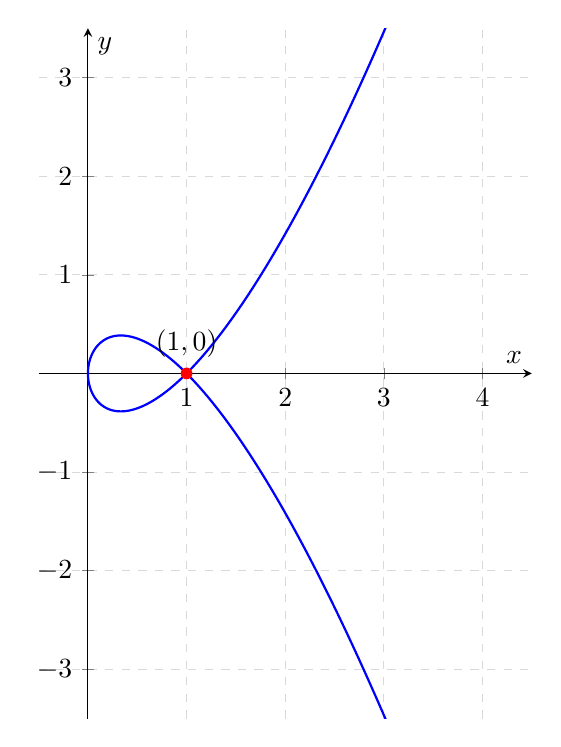
\begin{tikzpicture}
\begin{axis}[
    width=12cm,
    axis equal image,
    axis lines=middle,
    xlabel=$x$,
    ylabel=$y$,
    xmin=-0.5, xmax=4.5,
    ymin=-3.5, ymax=3.5,
    xtick={0,1,2,3,4},
    ytick={-3,-2,-1,0,1,2,3},
    grid=major,
    grid style={dashed, gray!30},
]
% Plot the curve using its parametric form
\addplot[
    variable=t, % This is the crucial fix
    domain=-2.1:2.1,
    samples=200,
    smooth,
    thick,
    blue,
]
({t^2}, {t^3-t});

% Add a node to mark the singularity
\node[circle, fill=red, inner sep=1.5pt, label={above:$(1,0)$}] at (axis cs:1,0) {};

\end{axis}
\end{tikzpicture}

We claim that $M_1$ is an \emph{immersed} submanifold. It suffices to show that the inclusion $i:M_1\hookrightarrow \mathbb{R} ^2$ induces injective differentials $\mathrm{d}_p i$ at each $p\in M_1$. Equivalently, we show that $\mathrm{d}_p i$ has trivial kernel. Let $v\in T_pM^1$ such that $\mathrm{d}_p i(v)=0$. Then in particular, if $f : \mathbb{R} ^2 \to \mathbb{R} $ is given by $f(x,y)=xy$, then $\mathrm{d}_p i(v)(f)=0$. Since $\mathbb{R} $ has trivial charts, a bais is given by just the usual partial derivatives
\[
	\mathrm{d}_p i(v)(f)=\sum_{i} v^i \left. \frac{\partial f\circ i}{\partial x^i} \right|_p=v^x y|_p + v^yx|_p=v^xp^y+v^yp^x
.\]
Of course the only case with $x=0$ is $(0,0)$, and the only cases with $y=0$ are $(0,0)$ and $(1,0)$. For all other cases, we have that $p^x,p^y \neq 0$, so $v=0$. We now specialize to these two cases.

In the case of $p=(1,0)$, we obtain that $v^y=0$, so we define a new map $f(x,y)=x$. Computing $\mathrm{d}_p i(v)(f)=v^x$ since the partials are $1$ and 0, and since this is 0, we have that $v^x=0$. This case also gets us that $v^x=0$ in the case $p=(0,0)$, since the partials are not dependent on $p$. Similarly, using $f(x,y)=y$ gives that $v^y=0$. Therefore, $v=0$ in all cases, and $\mathrm{d} _p i$ is injective. Therefore, $M_1$ is an immersed submanifold of $\mathbb{R} ^2$.

We claim that $M_0$ is not a submanifold in any manner. We will show that $M_0$ has a disconnected point at the origin, and thus it will locally be 0-dimensional at that point. However, the rest of the manifold is still a path, so it must be 1-dimensional by a similar argument to one given earlier, and thus the manifold will not have a well-defined dimension, and cannot be a manifold.

Note that $(0,0)$ solves $x^2(x-1)=y^2$. We will show that there is no nonzero positive $x,y<1$ with $(x,y)$ solving the problem. If $y=0$, then we either have $x=0$ or $x=1$, and $x=0$ is the case we have already discussed, and $x=1$ is not $x<1$. Therefore, we may take $y\neq 0$. Of course if $x=0$ then $y=0$ is forced, so we may also take $x\neq 0$. Therefore, we have $0<x,y<1$. We thus have $0<y^2<1$ and $0<x^2<1$. However, $x<1$ implies $x-1<0$, and thus $x^2(x-1)<0$. Therefore, we have
\[
	0>x^2(x-1)=y^2>0,
\]
a contradiction. Therefore, there are no nonzero $(x,y)$ with $0<x,y<1$ in $M_0$.
\end{proof}



\end{document}
